% Issues: Quote symbol, Algorithm2e
% \hyperpage{} command not creates when compiling index with makeindex engine.
% Page link: \hyperlink{page.2}{First page}

\documentclass[11 pt]{article}


% Packages.
\usepackage[margin=2.5cm]{geometry}
\usepackage[document]{ragged2e}
\usepackage[ruled, vlined]{algorithm2e}
\usepackage[table, x11names, svgnames]{xcolor}
\usepackage
{
	tkz-graph,
	pgfplots,
	hyperref,
	csquotes, % quotes: \enquote{}, \enquote*{}
	longtable,
	array,
	amsmath,
	imakeidx, % index, change compiler to MakeIndex then compile. Then compile again with XeLaTeX or PDFLaTeX.
	mathabx,
}

\usetikzlibrary{shadows}
\usetikzlibrary{arrows.meta, arrows}

\title{Assignment CSE201: Data Structure}
\author{\textbf{{\large Md. Kazi Iqbal Hossen}}\\\textbf{18ICTCSE065}\\\textbf{SHIICT, BSMRSTU}}


\hypersetup
{
	colorlinks = true,
	linkcolor = blue,
	filecolor = magenta,
	urlcolor = cyan,
	pdftitle = {CSE201 assignment},
	linktocpage = false,
	breaklinks = false,
	frenchlinks = false,
	bookmarks = true,
	hyperindex = true,
}


\renewcommand\contentsname{Sections \& Sub-Sections}
\makeindex

\begin{document}

\pagecolor{LightSlateGray}
\newcommand{\Exjobbsnummer}[1]{
\begin{tikzpicture}[overlay, remember picture]
\path (current page.north east) ++(-1,-1) node[below left] {{\small #1}};
\end{tikzpicture}
}

\newcommand{\Examensjobbspoang}[1]{
\begin{tikzpicture}[overlay, remember picture]
\path (current page.north east) ++(-1,-1.5) node[below left] {{\normalsize \scshape Examensarbete #1 HP}};
\end{tikzpicture}
}

\newcommand{\datum}[1]{
\begin{tikzpicture}[overlay, remember picture]
\path (current page.north east) ++(-1,-2.0) node[below left] {{\normalsize #1}};
\end{tikzpicture}}

\newcommand{\storlitentitel}[2]{
\center
\rule[0.2cm]{13cm}{0.1cm}
{ \huge \bfseries #1}\\[0.4cm] % Title of your document
{\Large \slshape #2}\\[0.4cm]
\rule[0.2cm]{13cm}{0.1cm}\\[3cm]

}

\newcommand{\Namn}[2]{
\begin{minipage}{0.4\textwidth}
\normalsize
\centering
#1 \textsc{#2}\\
\end{minipage}\\
}

\newcommand{\LoggaSwe}
{
	\textsc{\huge Bangabandhu Sheikh Mujibur Rahman Science and Technology University, Gopalganj \\[0.3cm] SHIICT}\\[0.7cm]
	
\includegraphics[scale=.3]{Pictures/0vtMuuSi_400x400.jpg}\\[1.5cm]
}

\newcommand{\LoggaEng}{
\textsc{\Huge BSMRSTU}\\[0.7cm]

\includegraphics[scale=.4]{Pictures/0vtMuuSi_400x400.jpg}\\[0.5cm]
}


\begin{titlepage}

\center 


\Exjobbsnummer{Version v03}

\datum{October 10, 2021}

\LoggaSwe

\storlitentitel{Assignment CSE201}{Data Structure}

\Namn{}{Md. Kazi Iqbal Hossen}
\Namn{ID:}{18ICTCSE065}
\Namn{Dept.}{CSE, 18-19}

\vfill

\end{titlepage}
%\textcolor{gray}{\rule{\textwidth}{2 pt}}
%\vfill
%\begin{center}
%	
\includegraphics[scale=0.4]{Pictures/0vtMuuSi_400x400.jpg} 
%\end{center}
\pagecolor{white}
\tableofcontents
\listoffigures
\pagebreak

\section{What is a data structure? What are the types of data structures? What are the notations of measurement of performance of an algorithm?}
\justify
{
\index{Definition of data structure}{\huge\textcolor{red}{\hspace{5 mm}D}}ata structure is a special way of organizing data in a computer so that we can use those efficiently later. Types of data structures means how the data structure implemented and how it looks like when comparing with the real world, how structured the skeleton that stayed beyond of that data structure, is it linear or non-linear? is it stack type or hierarchical tree type as well.\\
\index{Basic types of data-structure}The two basic types of data-structure:
\begin{enumerate}
	\item[$\blackdiamond$] Linear
	\item[$\blackdiamond$] Non-linear
\end{enumerate}
\index{Algorithmic notations}
To solve a problem we builds some different logic and algorithm but we don't know actually which algorithm is more efficient for our program in terms of holding less memory and shortest time. That's why we compare algorithms in a manner to find out best algorithmic approach that takes less memory and shortest time to make our program efficient. Due to respect of finding best algorithm there are so many approaches and they are denoted by some kind of mathematical notations. By those notations we measure the performance of an algorithm and scalability.\\
Some notations are:
\begin{enumerate}
	\item Big Theta notation $\theta(\textrm{ })$
	\item Big Ow notation $O(\textrm{ })$
	\item Big Omega notation $\omega(\textrm{ })$
\end{enumerate}
\index{Analysis graph by BIG O notation} Mostly used notation here is big Ow notation $O(\textrm{ })$. Here is a complexity analysis graph via big Ow notation $O(\textrm{ })$.
}
	\begin{figure}[h!]
	\begin{tikzpicture}
	
		\begin{axis} [
						axis lines = left,
						xlabel = $x$,
						ylabel = $f(x)$,
						legend pos = outer north east,
						xtick = {0, 1, 2,...,10},
						ytick = {0, 2,...,16}
					 ]
			\addplot[green, domain = 0:10] {1};
			\addplot[red, domain = 0:10] {x};
			\addplot[black, domain = 0:4] {x^2};
			\addplot[gray, domain = 0:4] {2^x};
			\addplot[blue, domain = 0:10] {log10(x)};
			\addplot[yellow, domain = 0:10] {x*log10(x)};
			
			\legend{$O(1) / C$: Constant, $O\left(n\right)$: Linear, $O\left(n^2\right)$: Quadratic, $O\left(2^n\right)$: Exponential, $O\left(log_{10}n\right)$: Logarithmic, $O\left(nlog_{10}n\right)$: Logarithmic Pro}
		\end{axis}
		
	\end{tikzpicture}
	\centering
	\caption{Complexity analysis graph due to respect of BIG $O$}
	\end{figure}

\pagebreak

\section{What is bubble sort? Write an algorithm for sorting an array of N elements using bubble sort. Sort this array using bubble sort: [15, 18, 4, 5, 2]}
\justify
{
\index{Bubble sort definition} Bubble sort is a very simple sorting algorithm which sort elements by just swapping two adjacent element is they are not in the correct order. Bubble sort has $O(n^2)$ as it's worst-case and average-case time complexity. Here is the algorithm of bubble sort:
}
\index{Bubble sort algorithm}
\begin{algorithm}
\DontPrintSemicolon
\KwData{An array of N elements.}
\KwResult{Sorted list.}
\Begin
{
$\textrm{Declare \& initialize variable i=0, j=0 and n}=\textrm{length(array)}$.\;
Set boolean swapped to false.\;
\For{i from 0 to n-1, increment by 1}
{
	\For{j from 0 to n-i-1, increment by 1}
	{
		\If{array$[j]$ is greater than array$[j+1]$}
		{
			Swap(array$[j]$, array$[j+1]$)\;
			Set swapped value to true.
		}
	}
	\If{not swapped}{exit from the loop.}
	\Else{Set swapped value to false again.}
}
}
\textbf{end}
\caption{Bubble Sort: optimized for boolean supported language.}
\end{algorithm}

\index{Bubble sort iteration steps}
Sorting the array [15, 18, 4, 5, 2] using bubble sort:
\begin{enumerate}
	\item After iteration 1: [15, 18, 4, 5, 2]
	\item After iteration 2: [15, 4, 18, 5, 2]
	\item After iteration 3: [15, 4, 5, 18, 2]
	\item After iteration 4: [15, 4, 5, 2, 18]
	\item After iteration 5: [4, 15, 5, 2, 18]
	\item After iteration 6: [4, 5, 15, 2, 18]
	\item After iteration 7: [4, 5, 2, 15, 18]
	\item After iteration 8: [4, 5, 2, 15, 18]
	\item After iteration 9: [4, 5, 2, 15, 18]
	\item After iteration 10: [4, 2, 5, 15, 18]
	\item After iteration 11: [4, 2, 5, 15, 18]
	\item After iteration 12: [4, 2, 5, 15, 18]
	\item After iteration 13: [2, 4, 5, 15, 18]
\end{enumerate}
\textcolor{blue}{Yep! Sorted using bubble sort.}

\pagebreak

\section{What are the types of linked list? Explain with diagram. Write and algorithm to delete element(node) from \enquote{pos} position in linked list}
\index{Linked list type definition}
\subsection{Type definition with diagram}
\justify
{
Types of linked list means looking structure of a linked list.\\
Types of linked list with diagram:
\begin{enumerate}
	\item Singly linked list, forward iteration only\\
	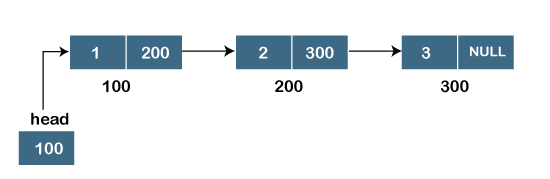
\includegraphics[scale=0.5]{Pictures/singly.png} 
	\item Double linked list, can iterate both forward and backward\\
	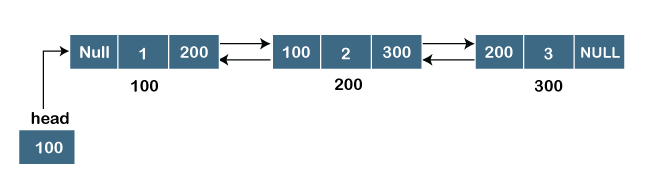
\includegraphics[scale=0.5]{Pictures/doubly.png} 
	\item Circular linked list, tail is linked with head, forward iteration only\\
	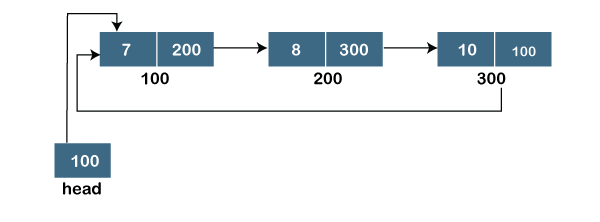
\includegraphics[scale=0.5]{Pictures/circular.png} 
	\item Double circular linked list, tail is linked with head, forward and backward both iteration supported\\
	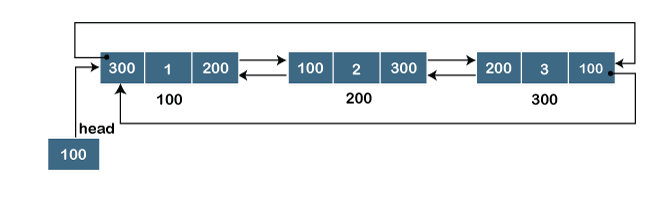
\includegraphics[scale=0.5]{Pictures/doubly circular.png}
\end{enumerate}
}
\pagebreak
\index{Algorithm to delete a node from linked list}
\subsection{Algorithm to delete a node from \enquote{pos} index}
\begin{algorithm}
\DontPrintSemicolon
\KwData{Head of the linked list and \enquote{pos} of that node which to delete.}
\KwResult{Modified list.}
\Begin
{
\If{head is null or next node of head is null and \enquote{pos} $\geq$ 1}
{
	Return null with \textcolor{red}{error} message \enquote{NullPointerException} and terminate the program.
}
Declare and initialize prev = head and curr = head.next node respectively\;
Now declare and initialize idx = 0 for loop over the linked list\;
\While{idx+1$\neq$pos and curr$\neq$null}
{
	Forward prev node one step, $prev = prev.next$\;
	Forward curr node one step, $curr = curr.next$\;
	Increment idx by 1.
}
Set prev.next node value to curr.next, $prev.next = curr.next$\;
De-allocate space for $curr$ node and free the memoey.\;
Exit with success code 0.
}
\textbf{end}

\caption{Delete a node from \enquote{pos}}
\end{algorithm}

\pagebreak

\section{Define the properties of complete binary tree. Create a tree from given orders of traversals- Preorder: \{11, 5, 3, 8, 16, 14, 18, 17, 20\}, Inorder: \{3, 5, 8, 11, 14, 16, 17, 18 , 20\}}

\subsection{Properties of complete binary tree}
\index{Properties of complete binary tree}
A binary tree is a hierarchical tree type data structure where every node has at most 2 children and in a proper\textbackslash complete binary tree every internal nodes has exactly 2 child nodes. \\
Properties of binary tree:
\begin{itemize}
	\item Special type of binary tree which every level, except possibly the last, is completely filled and all nodes are as far left as possible.
	\item At each level, there are exactly $2^l$ child nodes at level \enquote*{l} where root is assumed as level 1.
	\item Height of that tree is $\log(n+1)$ where n is the number of nodes in the tree.
\end{itemize}

\subsection{Constructed binary tree}
\index{A binary tree constructed from given traversals}
Preorder: \{11, 5, 3, 8, 16, 14, 18, 17, 20\}\\
Inorder: \{3, 5, 8, 11, 14, 16, 17, 18 , 20\}
\begin{figure}[h!]
	\begin{tikzpicture}[edge from parent/.style={draw, thick}]
		\node[fill=gray!80, circle, draw](11) {11} [grow=down]
	 		child {node[fill=gray!60, circle, draw](5) {5}
	 			child {node[fill=gray!40, rectangle, draw](3) {3}}
	 			child {node[fill=gray!40, rectangle, draw, right of=3](8) {8}}}
	 		child {node[fill=gray!60, circle, draw](16) {16}
	 		    child {node[fill=gray!40, rectangle, draw, right of=8](14) {14}}
	 			child {node[fill=gray!40, circle, draw](18) {18}
	 				child {node[fill=gray!20, rectangle, draw](17) {17}}
	 				child {node[fill=gray!20, rectangle, draw](20) {20}}}};
	\end{tikzpicture}
\centering
\caption{Binary tree constructed from given traversals}
\end{figure}

\pagebreak

\section{Convert the following infix equation to postfix equation using stack:\\$(A+B\textrm{ }\hat{ }\textrm{ }D)/(E-F)+G$}

\index{Infix notation to postfix notation with an example}
\begin{center}
\rowcolors{2}{green!30}{green!60}
\arrayrulecolor{white}
\begin{longtable}{|| m{2.8 em} || m{5 em} m{5 em} m{9 em} ||}
	\hline
	\rowcolor{black}
	\textbf{\textcolor{white}{Serial}} & \textbf{\textcolor{white}{Char}} & \textbf{\textcolor{white}{Stack}} & \textbf{\textcolor{white}{Equation}} \\
	\hline\hline\hline\hline
	1 & $($ & $($ &  \\
	2 & A & $($ & A \\
	3 & $+$ & $(+$ & A \\
	4 & B & $(+$ & AB \\
	5 & $\hat{ }$ & $(+\textrm{ }\hat{ }$ & AB \\
	6 & D & $(+\textrm{ }\hat{ }$ & ABD \\
	7 & ) & & ABD$\textrm{ }\hat{ }+$ \\
	8 & / & / & ABD$\textrm{ }\hat{ }\textrm{ }+$ \\
	9 & ( & $/($ & ABD$\textrm{ }\hat{ }\textrm{ }+$ \\
	10 & E & $/($ & ABD$\textrm{ }\hat{ }\textrm{ }+$E \\
	11 & - & $/(-$ & ABD$\textrm{ }\hat{ }\textrm{ }+$E \\
	12 & F & $/(-$ & ABD$\textrm{ }\hat{ }\textrm{ }+$EF \\
	13 & ) & $/$ & ABD$\textrm{ }\hat{ }\textrm{ }+$EF$-$ \\
	14 & + & $+$ & ABD$\textrm{ }\hat{ }\textrm{ }+$EF$-/$ \\
	16 & G & $+$ & ABD$\textrm{ }\hat{ }\textrm{ }+$EF$-/$G \\
\end{longtable}
\end{center}
Final postfix equation: $ABD\textrm{ }\hat{ }+EF-/G+$

\pagebreak

\section{What is the difference between sequential(linear) search and binary search? Show the steps of searching element \enquote*{5} using binary search technique in [2, 5, 8, 15, 20]}
\index{Difference between linear search \& binary search}
\justify
{
Linear search is a searching approach that tries to find out an element in a given list\textbackslash array sequentially from start to end where a binary search approach always grab the middle element in the list and try to match it with the given key, if founds then return its index or recursively do the same approach until left index is not greater than of right index. In binary search, list\textbackslash array must be sorted.\\
}
\index{Steps to search a certain number in binary search approach}
Searching \enquote*{5} in [2, 5, 8, 15, 20], steps:
\begin{enumerate}
	\item Set $key = 5$.
	\item First iteration:
		\begin{enumerate}
			\item left = 0
			\item right = length(list) = 5
			\item $mid = floor\_int\left(\frac{left+right}{2}\right) = 2$
			\item list[mid] is greater than key. So, $right = mid -1 = 1$
		\end{enumerate}
	\item Second iteration:
		\begin{enumerate}
			\item left = 0
			\item right = 1
			\item $mid = floor\_int\left(\frac{left+right}{2}\right) = 0$
			\item list[mid] is less than key. So, $left = mid+1 = 1$
		\end{enumerate}
	\item Third iteration:
		\begin{enumerate}
			\item left = 1
			\item right = 1
			\item $mid = floor\_int\left(\frac{left+right}{2}\right) = 1$
			\item list[mid] is equal to the key. Return mid as index with success code 0.
		\end{enumerate}
\end{enumerate}

\pagebreak

\section{Explain merge sort using an example.}
\index{Definition of merge sort}
\justify
{
Merge sort is an efficient sorting algorithm that follows Divide and Conquer algorithm to sort the given list of elements. Technique is recursively divide the given list in two halves until we obtain a certain stage where the length of the list becomes only 1. After that, merge those individual arrays in sorted manner till we combines the total list. Here is a pictorial demonstration available that gives a better understanding with an example of list: [38, 27, 43, 3, 9, 82, 10]\\
}
\index{A merge sort illustration figure}
\begin{figure}[h!]
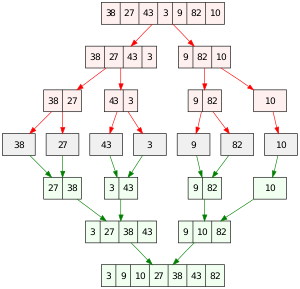
\includegraphics[scale=0.7]{Pictures/300px-Merge_sort_algorithm_diagram.svg.png}
\centering
\caption{Merge sort illustration}
\end{figure}
\index{Steps to sort a list using merge sort algorithm}
Here, considering a list of integers and recursively divide it into two-halves until the length of divided list becomes 1, then contineously merge them in sorted manner untill we reach the exact length as original input.
\begin{enumerate}
	\item[Step 1:] [38, 27, 43, 3, 9, 82, 10]
	\item[Step 2:] [38, 27, 43, 3] [9, 82, 10]
	\item[Step 3:] [38, 27] [43, 3] [9, 82] [10]
	\item[Step 4:] [38] [27] [43] [3] [9] [82] [10]
	\item[Step 5:] [27, 38] [3, 43] [9, 82] [10]
	\item[Step 6:] [3, 27, 38, 43] [9, 10, 82]
	\item[Step 7:] [3, 9, 10, 27, 38, 43, 82]
\end{enumerate}
\textcolor{blue}{Yep! the list is sorted.}

\pagebreak

\section{Consider the weighted graph G in Fig-1. Suppose the nodes are stored in an array data as follows: [X, Y, S, T]. (a) Find the weight matrix W of G. (b) Find the matrix Q of shortest paths using Warshall's algorithm.}
\index{A simple graph}
\begin{center}
% \usetikzlibrary{shadows}
% \usetikzlibrary{arrows.meta, arrows}

	\tikzset{myNode/.style={draw, circle, white, radius=2pt, top color=red!40, bottom color=red!100, circular drop shadow={black!30}}, myEdge/.style={-{Stealth[open, round]}, very thick, green}} % thin, thick, very thick, fill=color_name removed. font=\itshape or \ttfamily.
	\tikz
	{
		% Vertices
		\node(Y) [myNode] at (2, 1) {\textbf{Y}};
		\node(X) [myNode] at (-2, 1) {\textbf{X}};
		\node(T) [myNode] at (-2, -1) {\textbf{T}};
		\node(S) [myNode] at (2, -1) {\textbf{S}};
		
		% Edges
		\draw[myEdge] (Y) to node[auto, swap, black, font=\ttfamily] {\textbf{3}} (X);
		\draw[myEdge] (Y) to node(2) [auto, black, font=\ttfamily] {\textbf{2}} (S);
		\draw[myEdge] (T) to node[auto, black, font=\ttfamily] {\textbf{4}} (S);
		\draw[myEdge] (T) to node[auto, black, font=\ttfamily] {\textbf{6}} (X);
		\draw[myEdge] (T) to node[auto, black, font=\ttfamily] {\textbf{1}} (Y);
		\draw[myEdge] (X) to[out=40, in=90+50] node[auto, black, font=\ttfamily] {\textbf{7}} (Y);
		\draw[myEdge] (S) to[out=-140, in=-40] node[auto, swap, black, font=\ttfamily] {\textbf{5}} (T);
		
		\node[draw, black, right=1cm, text width=6cm, font=\itshape, fill=green!10] at (2) {\textbf{Find out the shortest path of this graph using Warshall's algorithm.}};
	}

\end{center}

%\begin{figure}[hbtp]
%\centering
%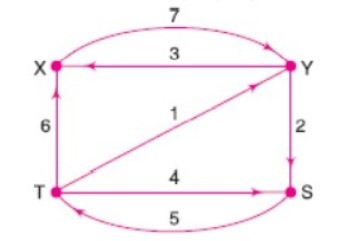
\includegraphics[scale=0.5]{Pictures/Screenshot_2.jpg}
%\caption{A directed graph}
%\end{figure}

\index{Weight matrix illustration}
\subsection{Weight matrix}
$$
\textrm{Weight matrix of G, W }=
\begin{Vmatrix}
	  & X & Y & S & T\\
	X & 0 & 7 & 0 & 0 \\
	Y & 3 & 0 & 2 & 0 \\
	S & 0 & 0 & 0 & 5 \\
	T & 6 & 1 & 4 & 0 \\
\end{Vmatrix}
$$
	
\subsection{Finding shortest path using Warshall's algorithm}
\index{Warshall's algorithm illustration}
$$
Q_0=
\begin{bmatrix}
	0 & 7 & \infty & \infty \\
	3 & 0 & 2 & \infty \\
	\infty & \infty & 0 & 5 \\
	6 & 1 & 4 & 0 \\
\end{bmatrix}
$$
\vspace{0.5cm}
$$
Q_X=
\begin{bmatrix}
0 & 7 & \infty & \infty \\
3 & 0 & 2 & \infty \\
\infty & \infty & 0 & 5 \\
6 & 1 & 4 & 0 \\
\end{bmatrix}
\hspace{2cm}
Q_Y=
\begin{bmatrix}
0 & 7 & 9 & \infty \\
3 & 0 & 2 & \infty \\
\infty & \infty & 0 & 5 \\
4 & 1 & 3 & 0 \\
\end{bmatrix}
$$
\vspace{0.5cm}
$$
Q_S=
\begin{bmatrix}
0 & 7 & 9 & \infty \\
3 & 0 & 2 & 7 \\
\infty & 0 & 0 & 5 \\
4 & 1 & 3 & 0 \\
\end{bmatrix}
\hspace{2cm}
Q_T=
\begin{bmatrix}
0 & 7 & 9 & \infty \\
3 & 0 & 2 & 7 \\
11 & 6 & 0 & 5 \\
4 & 1 & 3 & 0 \\
\end{bmatrix}
$$

Ultimately the shortest path: 
$
\textrm{Q}=
\begin{Vmatrix}
0 & 7 & 9 & \infty \\
3 & 0 & 2 & 7 \\
11 & 6 & 0 & 5 \\
4 & 1 & 3 & 0 \\
\end{Vmatrix}
$

\pagebreak
%\hyperlink{page.2}{First page}
%\hyperlink{page.10}{Last page}
\printindex

\end{document}
